\section{Fun With Filters}
\label{lab_filters}

%\makelabheader %(Space for student name, etc., defined in master.tex)

\bigskip

\begin{enumerate}[wide]

\item The circuit below is called a filter, because it ``filters out'' some frequencies but not others.  Connect $V_{IN}$ to your function generator, and measure $V_{OUT}/V_{IN}$ for different frequencies.  (Use 10~Hz, 30~Hz, 100~Hz, etc., up to 100~kHz .)  Plot $V_{OUT}/V_{IN}$ vs. the frequency $f$ using Excel, and include a printout of the graph taped into your notebook.  \label{part_low_pass_RC}
\begin{center}
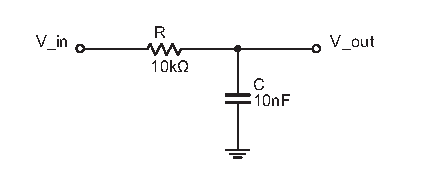
\includegraphics{filters/low_pass_filter_RC.eps}
\end{center}

\item A low pass filter filters out high frequencies, allowing low frequencies to ``pass through.''  A high pass filter filters out low frequencies, allowing high frequencies to pass through.  Which kind of filter did you just build?  

\item Plot your data from part~\ref{part_low_pass_RC} for $V_{OUT}/V_{IN}$ in decibels vs. $f$, where $f$ is plotted on a log scale axis.  Show on the graph the frequency at which $V_{OUT}/V_{IN}=-3$~dB, called the ``cutoff frequency,'' $f_C$.  Is your value of $f_C$ consistent with the expression you derived for $V_C$ in your homework?  Check your graphs with your instructor now to make sure you're on the right track.

\item Measure the phase shift $\phi$ between $V_{OUT}$ and $V_{IN}$ as a function of $f$, and make a rough plot of it.  (You don't need many data points for this, just enough to give some idea of what $\phi$ does for $f \ll f_C$, $f = f_C$, and $f \gg f_C$.)

\item Design and build a \textit{high pass} filter by switching the positions of the capacitor and the resistor in your previous circuit.  Change the value of the capacitor so that the cutoff frequency is 100~Hz.  Test your filter by recording $V_{OUT}/V_{IN}$ vs. $f$ and plotting the result in decibels on a logarithmic frequency scale as before.  

\item You can also build filters using resistors and inductors.  Is the filter pictured below a high pass or a low pass filter?  Predict its cutoff frequency, and then test your prediction with a measurement.
\begin{center}
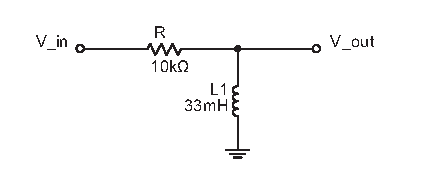
\includegraphics{filters/high_pass_filter_LR.eps}
\end{center}

\item Sketch how you would build a low pass filter using an inductor.  If you wanted your filter to use a 10~k$\Omega$ resistor, what value of $L$ would be required for a cutoff frequency of 10~Hz?  What would be the physical size of such an inductor?  By contrast, how big a capacitor would you need to make it work?  (This is why in real life most filters are made using capacitors instead of inductors.  Filters made using inductors are good for blocking very high radio frequencies called RF; for this reason inductors are sometimes called ``RF chokes.'')  

\item When you set the ``coupling'' on channel 1 or channel 2 of your oscilloscope to ``AC'' instead of ``DC,'' you are actually filtering the input.  Does ``AC coupling'' apply a low-pass filter or a high-pass filter?  Take some measurements to determine the exact cutoff frequency of this filter.  You should find that it's in the neighborhood of about 1~Hz.

\item Design a ``band pass filter'' that passes frequencies between 20 Hz and 20 kHz (roughly the audio range of human hearing).  Do this by building a high-pass RC filter and a low pass RC filter and hooking the output of one to the input of the other.  (Hint: you will want your first resistor to be about 10~k$\Omega$, and your second resistor to be about 100~k$\Omega$.  Why?)   Test your filter by making a graph of $V_{OUT}/V_{IN}$ vs. frequency.

\item Use your scope to look carefully at the output of your DC 5 volt power supply.  In particular, switch to ``AC coupling'' and crank up the scale to look at small deviations of the voltage.  What does it look like?  Is there a single dominant frequency in this ``noise''?  What else do you see in the signal?  (You did this before, in Lab~\ref{lab_oscilloscope}.  This is just a reminder.)

\item Design a low-pass filter that will effectively filter out as much of this unwanted ``noise'' and interference as possible, to produce something closer to a clean DC output.  Build it and test it, and draw what the output looks like.  What should be the cutoff frequency of this filter?  \textit{Important note:} for this exercise, you will need to ground the end of your filter to a CLEAN grounding point.  It turns out that the ``ground'' on your circuit boards is probably noisy as hell.  (Measure it with the scope, in fact.  How noisy is it?)  Use a ground on your oscilloscope instead.

\item The circuit below shows an easy way to add a DC offset (Also called a ``DC bias'') to an AC signal.  Use the principle of superposition to analyze this circuit, shorting out $V_{IN}$ and $V_{DD}$.  In each case, what is $V_{OUT}$ for both very high and very low frequencies?  Build it and test your predictions.
\begin{center}
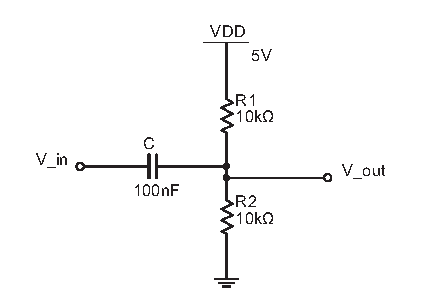
\includegraphics{filters/DC_biasing.eps}
\end{center}

\item The circuit below is called a resonance filter.  Make a plot of $V_{OUT}/V_{IN}$ vs. $f$, paying close attention to the response at $f \approx 2.5$~kHz.  Also plot the phase shift $\phi$ between $V_{OUT}$ and $V_{IN}$ as a function of $f$. 
\begin{center}
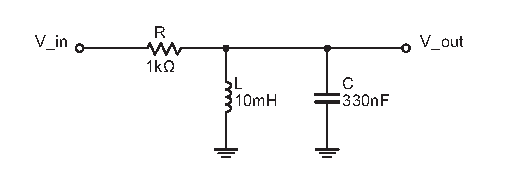
\includegraphics{filters/LC_resonance_filter.eps}
\end{center}

\item How would you modify this circuit to give a resonance frequency of 5~kHz?   Build it and test your prediction.


\end{enumerate}

\textbf{Possible Exam Questions:}

\begin{itemize}

\item Design a band pass filter between 400~Hz and 1~MHz, using one capacitor and one inductor, plus resistors.

\item Design a resonance filter with a resonance frequency of 1~kHz. 

\item Design a low-pass filter using a capacitor and a resistor with a $-3$~dB point of 4.7~kHz.

\item Show how to use a capacitor and two resistors to add a 2 volt DC offset to an AC signal.  What values of $R$ and $C$ are required for your circuit to work well at 3~kHz?

\item A low-pass filter uses a 22~nF capacitor and a 4.7~kΩ resistor.  What is the ratio $V_{OUT}/V_{IN}$, in dB, at a frequency of 80~kHz?

\end{itemize}





